

\documentclass[12pt]{article}
\usepackage{subfig}
\usepackage[english]{babel}
\usepackage[utf8x]{inputenc}
\usepackage[T1]{fontenc}
\usepackage{amsmath}
\usepackage{graphicx}
\usepackage{pstricks,pst-node}
\usepackage{stmaryrd}
\usepackage{gastex}
\usepackage{comment}
\usepackage{xcolor}
\usepackage{listings}
\usepackage{float}
\usepackage{url}
\usepackage[margin=1.3in]{geometry}
\usepackage[colorinlistoftodos]{todonotes}
\usepackage{wrapfig}
\usepackage{fullpage}
\usepackage{indentfirst}
\usepackage{pgfgantt}

\usepackage{tikz-uml}


\catcode`\_=12

\definecolor{mGreen}{rgb}{0,0.6,0}
\definecolor{mGray}{rgb}{0.5,0.5,0.5}
\definecolor{mPurple}{rgb}{0.58,0,0.82}
\definecolor{backgroundColour}{rgb}{0.95,0.95,0.92}

\lstdefinestyle{CStyle}{
    backgroundcolor=\color{backgroundColour},   
    commentstyle=\color{mGreen},
    keywordstyle=\color{magenta},
    numberstyle=\tiny\color{mGray},
    stringstyle=\color{mPurple},
    basicstyle=\footnotesize,
    breakatwhitespace=false,         
    breaklines=true,                 
    captionpos=b,                    
    keepspaces=true,                 
    numbers=left,                    
    numbersep=5pt,                  
    showspaces=false,                
    showstringspaces=false,
    showtabs=false,                  
    tabsize=2,
    language=C
}


\begin{document}

\begin{titlepage}

\newcommand{\HRule}{\rule{\linewidth}{0.5mm}} 
\center


\textsc{\Large Cahier des charges}\\[0.5cm]

\HRule \\[0.4cm]
{\huge \bfseries Project of Gestural Interaction}\\[0.4cm] 
\HRule \\[1.5cm]


\begin{minipage}{0.4\textwidth}
\begin{flushleft} \large
\emph{Equipe:}\\~\\
Qingyuan \textsc{Yao}\\
Alan \textsc{Adamiak}\\
David \textsc{Leconte}\\
\end{flushleft}
\end{minipage}
~
\begin{minipage}{0.4\textwidth}
\begin{flushright} \large
\emph{Encadrants:} \\~\\
Gilles \textsc{Bailly}\\~\\~\\
\end{flushright}
\end{minipage}\\[2cm]



\includegraphics[scale=0.5]{logo.png}\\[1cm] 

\vfill

\end{titlepage}




%DEBUT DU DOC 
\topskip0pt

\newpage

\renewcommand{\contentsname}{Table of Contents}
\tableofcontents
\newpage


\section{Introduction}
This is a project of 3 students in the first year of our master degree at Sorbonne Université under the guidance or Mr. Bailly.

The purpose of this project is to compare gestural interaction with keyboard input. We will compare the two primarily on execution speed and learning speed. In order to do that, we will make an interactive survey to record and gather input data from users and perform analysis based of that data. 

We hope this research project would prove the superiority of keyboard input and serves as an counterargument for papers that overestimate gestural interaction.

Down below, you will find the explanations on each stage of our project and how we plan to tackle them.

\section{Definitions}
Firstly, we would like to specify on the terms we use and comparisons we'll make, as there exists multiple types of gestural input. 

\subsection{Keyboard Input}
The keyboard input should come from a physical keyboard, with at least 26 Latin letters and modifier keys such as shift, control (command on Mac), alt, etc.

\subsection{Gestural Input}
The gestural input consists actions with only one pointer and it should come from a mouse or a touch-pad. Touch screen input is not considered in this project.

\subsection{Platform}
In order to test the speed of both types of input, the devices on which the test is to be done are required to have both input methods available. Ideally, all tests should be done on a computer with a keyboard and a mouse (or a touch-pad).

\section{Stages}

The project will be carried out in 5 stages, some stages can be done in parallel with others, and the previous 3 stages would be repeated at least twice in order to optimise collected data.

\subsection{Modeling (Input Design and Data Structure)}
A set of actions, ranging from copy-pasting to spatial movement would be defined as commands that will be activated with a gestural interaction as well as a keyboard input. 

The commands and inputs should be related and intuitive enough for everyday use as such is what we intend to simulate.

It's best to also define the data structure. The data to collect would be combination of input time, the evolution of input speed, precision, parameters on the users, etc.

\textbf{Plan of delivery: }By the end of this stage, all the gestures and keystrokes to use would be decided as well as the data structure.

\subsection{Interactive Test}
The program will be a web application coded in JavaScript, it would be hosted on a lip6 server for more people to access and take the test. The gamification of the survey is an option to consider if time allows

\subsubsection{Direct Commands}
The first part of the test would be command with specific actions such as "Click Control X to execute" or "Draw X to execute"

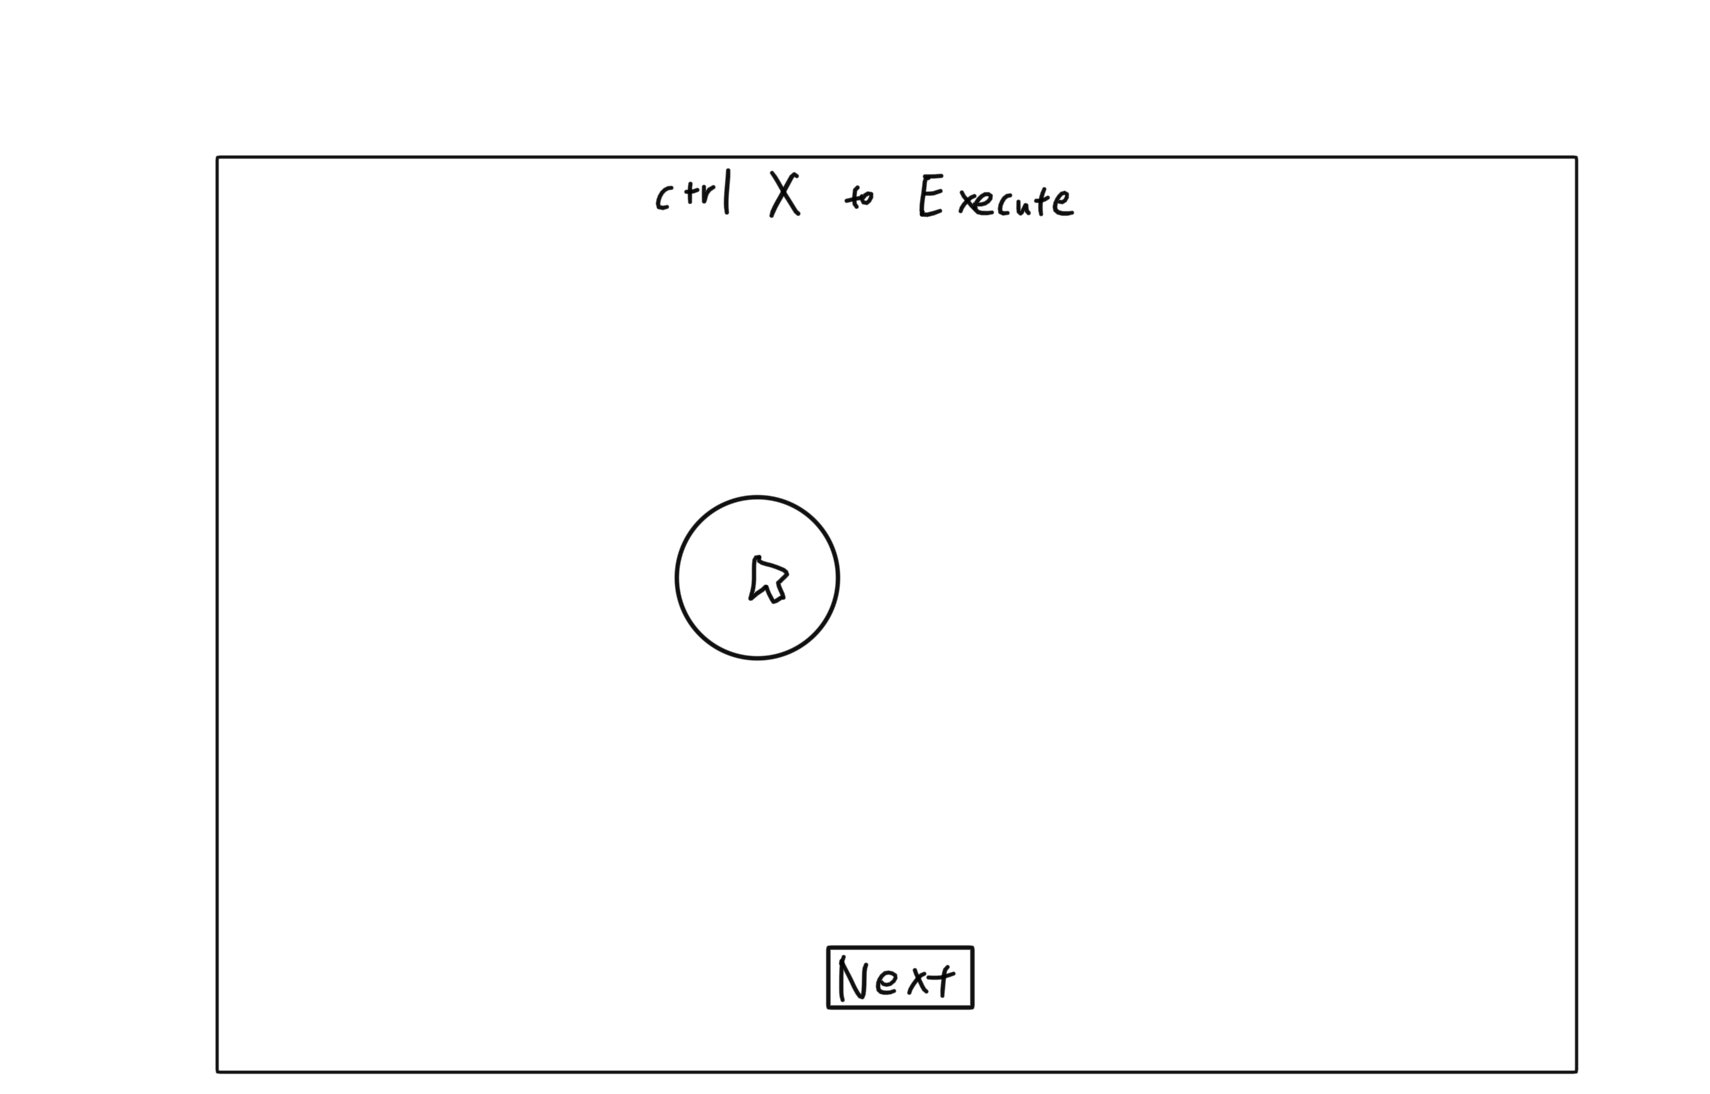
\includegraphics[scale=0.15]{click.jpg}

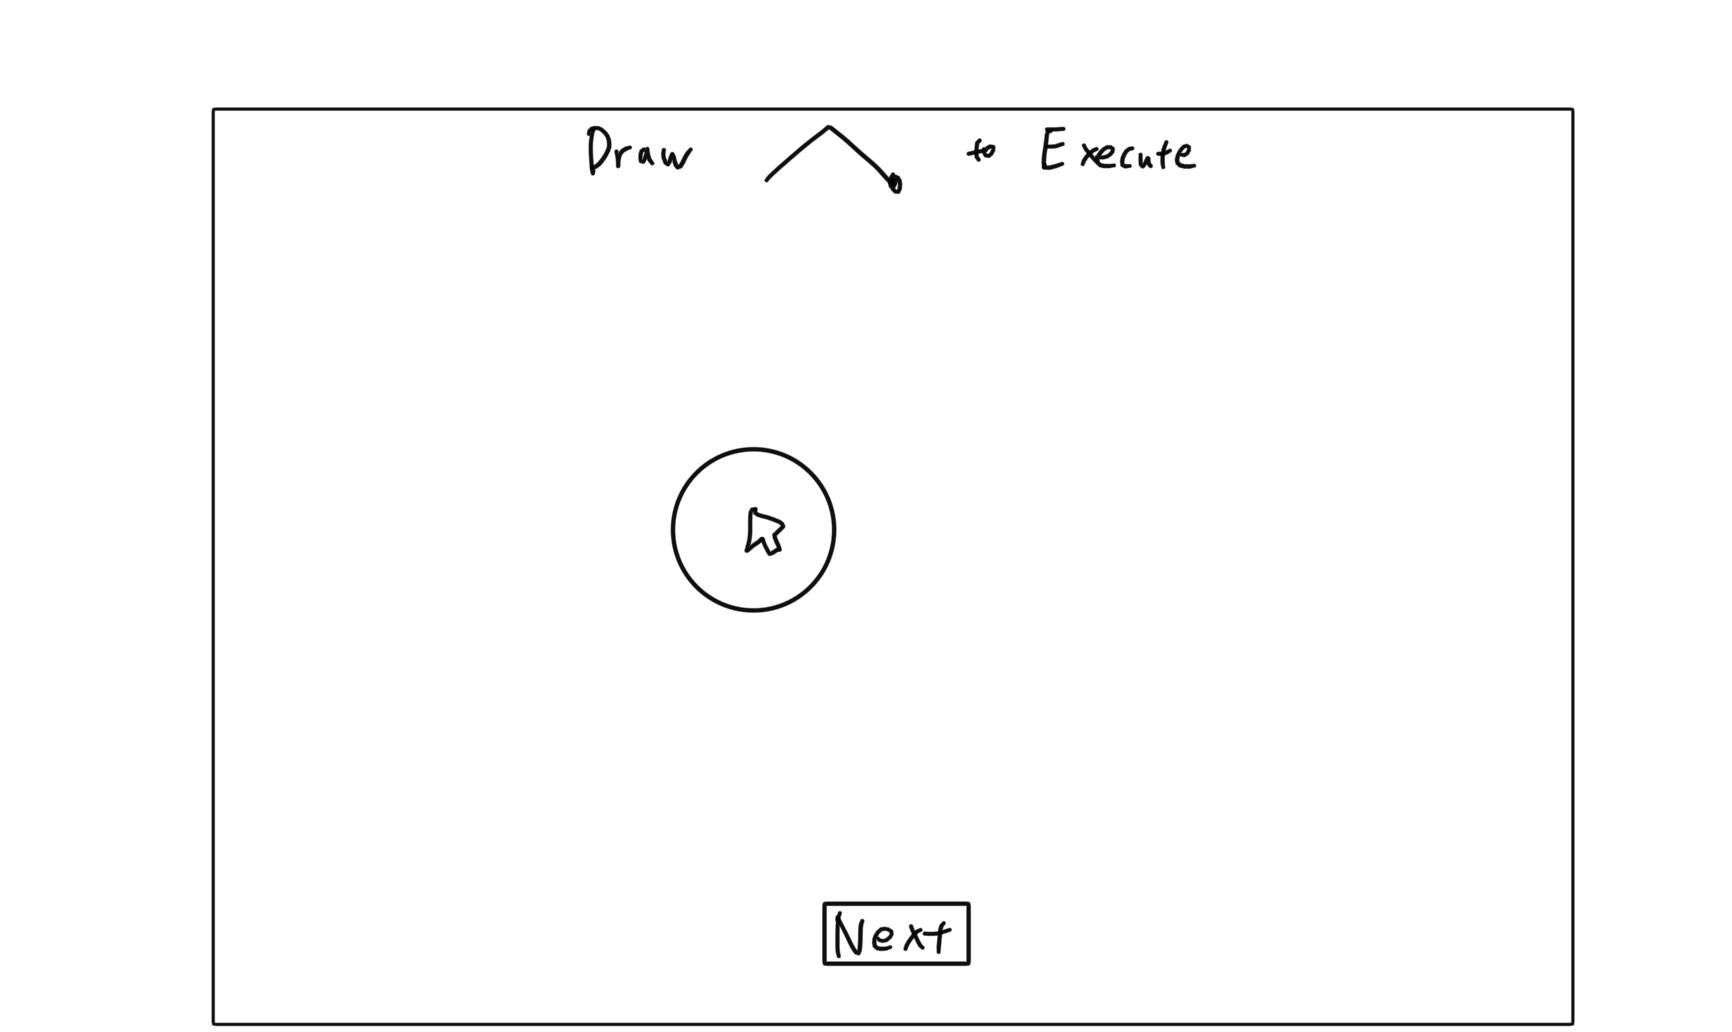
\includegraphics[scale=0.15]{draw.jpg}

\subsubsection{Natural Commands}
The second part is set out to test the learning speed for both types of input, so instead of showing "Click Control X to execute", the command would simply be "Execute"

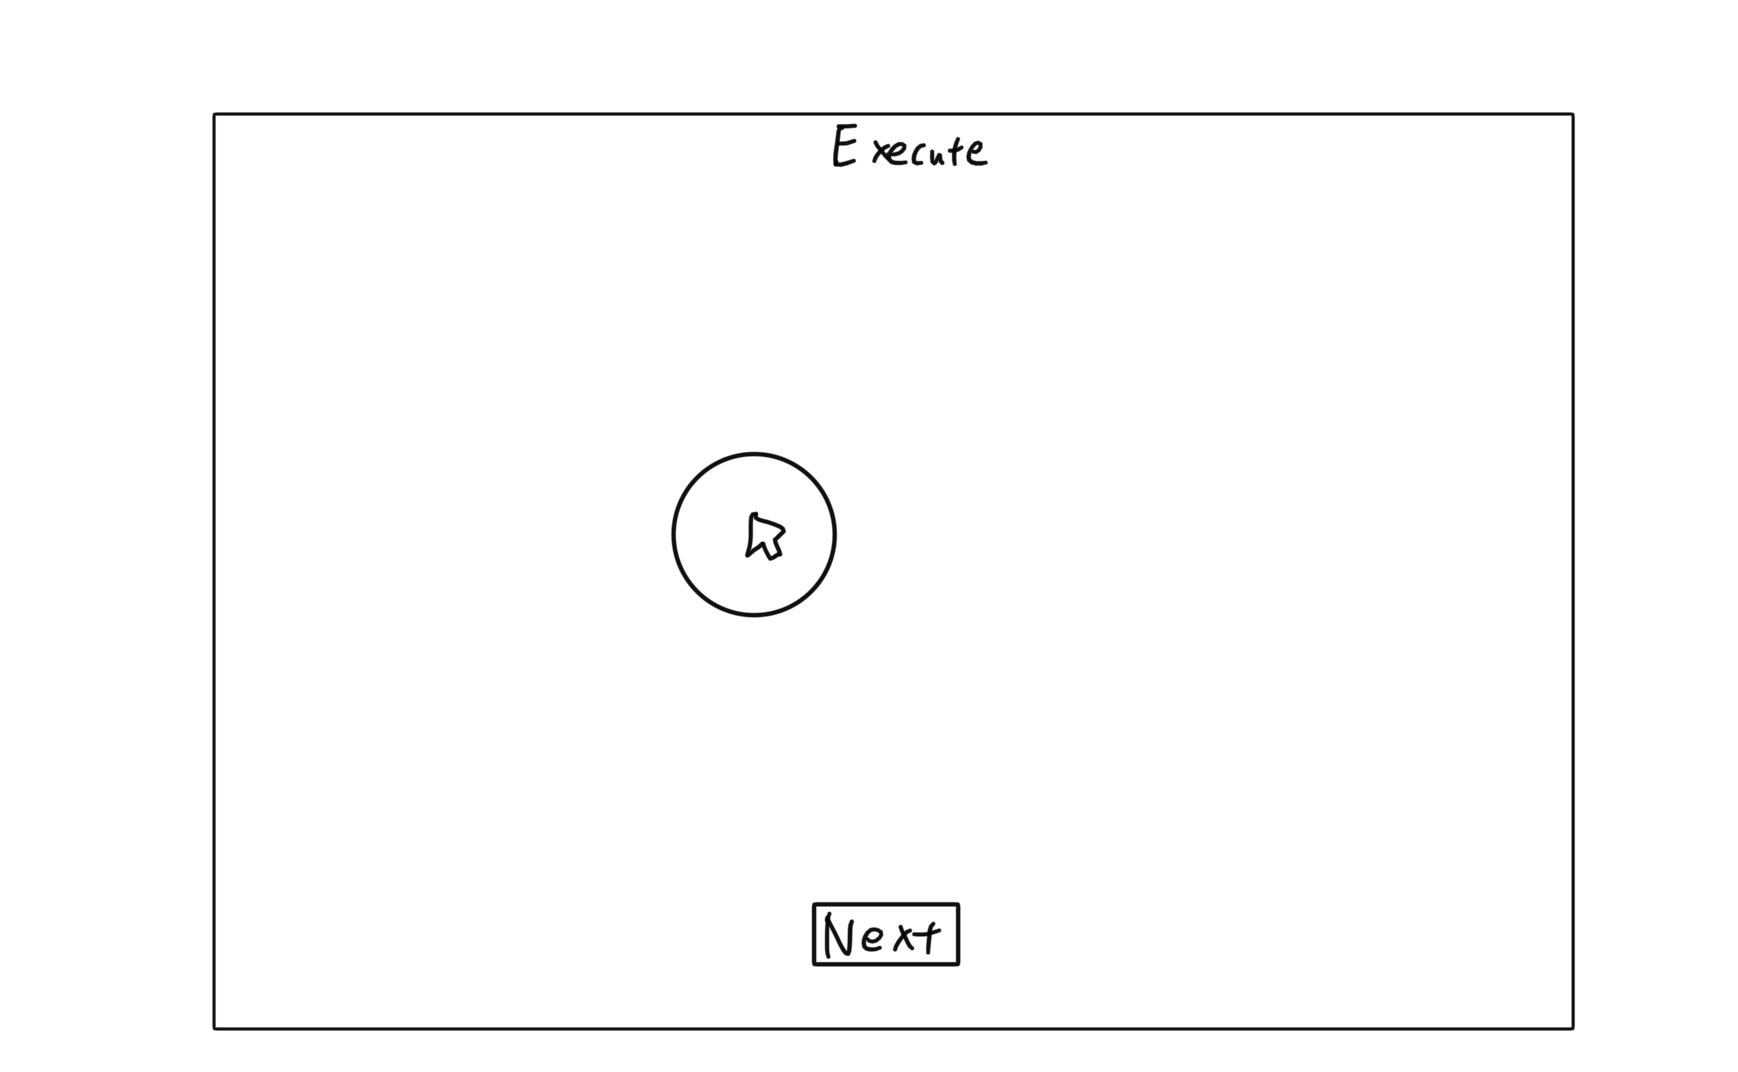
\includegraphics[scale=0.15]{x.jpg}

\subsubsection{Input Recognition}
One of the difficulties of programming the test would be the implementation of the recognizers for keyboard and gestural input. The rocognizers would take in the input and return true or false after being compared with the required command.

\subsubsection{Sequence Diagram}
The sequence diagram down below illustrate how a user (Bob) would interact with the program and how the program would respond.

\begin{center}
\begin{tikzpicture}
\begin{umlseqdiag}
\umlactor[class=Actor]{Bob}
\umlobject[class=UI]{u}
\umlobject[class=Key Recognizer]{k}
\umlobject[class=Gesture Recognizer]{g}

\begin{umlcall}[dt=5, op=Connect to website, type=synchron]{Bob}{u}
\begin{umlcall}[dt=5, op=Show info]{u}{Bob}
\end{umlcall}

\begin{umlcall}[op=Agree, type=synchron]{Bob}{u}
\begin{umlcallself}[op=Start test]{u}
\end{umlcallself}
\end{umlcall}

\begin{umlfragment}[type=loop]
    \begin{umlcall}[dt=-2, op=Show command]{u}{Bob}
    \end{umlcall}
    \begin{umlcall}[op=Keyboard input, type=synchron]{Bob}{u}
        \begin{umlcall}[padding=-1, op=Pass input, type=synchron, return=Return recognition]{u}{k}
            \begin{umlcallself}[op=Recognition]{k}
            \end{umlcallself}
        \end{umlcall}
        \begin{umlfragment}[type=alt, label=true, inner xsep=4]
            \begin{umlcall}[op=Next test, type=synchron, type=return]{u}{Bob}
            \end{umlcall}
            \umlfpart[false]
            \begin{umlcall}[op="Plese retry", type=synchron, type=return]{u}{Bob}
            \end{umlcall}
        \end{umlfragment}
    \end{umlcall}
\end{umlfragment}

\begin{umlfragment}[type=loop]
    \begin{umlcall}[dt=5, op=Show command]{u}{Bob}
    \end{umlcall}
    \begin{umlcall}[op=Gestural input, type=synchron]{Bob}{u}
        \begin{umlcall}[padding=-1, op=Pass input, type=synchron, return=Return recognition]{u}{g}
            \begin{umlcallself}[op=Recognition]{g}
            \end{umlcallself}
        \end{umlcall}
        \begin{umlfragment}[type=alt, label=true, inner xsep=4]
            \begin{umlcall}[op=Next test, type=synchron, type=return]{u}{Bob}
            \end{umlcall}
            \umlfpart[false]
            \begin{umlcall}[op="Plese retry", type=synchron, type=return]{u}{Bob}
            \end{umlcall}
        \end{umlfragment}
    \end{umlcall}
\end{umlfragment}

\begin{umlcall}[op="Thanks", type=synchron, type=return]{u}{Bob}
\end{umlcall}
\end{umlcall}

\end{umlseqdiag}

\end{tikzpicture}
\end{center}

\textbf{Plan of delivery: }By the end of this stage, the program which realizes the functionalities and steps of sequence diagram would be finished. The gamification is a surplus.

\subsection{Tests}
The test will be carried out online, and ideally, people of all socio-professional background would participate.

\textbf{Plan of delivery: }By the end of this stage, the estimated number of participants should have finished taking the test.


\subsection{Analysis}
After gathering enough data from the test. We will analyse the data in order to compare the execution speed and learning speed for both inputs based the data harvested during the experiment.

The data would be manipulated in Python.

Realization of the learning curve from the data would be a plus for the analysis.

\textbf{Plan of delivery: }By the end of this stage, conclusions would be drawn in order to write the report.

\subsection{Report}
After the analysis, a report will be redacted to explain in details the 5 previous stages, including the references we've used, the decisions we've made, the implementation we've done and the results we've obtained

\textbf{Plan of delivery: }By the end of this stage, the report would be finished.

\section{Progress Estimation and Tasks Distribution}
We estimate the project to be finished before the end of May 2022, which gives us approximately 4 months. A detailed estimation and task distribution is specified down below:

\begin{enumerate}
    \item \textbf{Research \& Modeling:} 2+1 weeks, 1-2 persons
    \item \textbf{Building the test website:} 1 month + 2 weeks, 2-3 persons
    \begin{itemize}
        \item UI, 1 week
        \item Recognizers, 2 weeks
        \iten Server 1 week
        \item Readjustment and optimisation 1-2 weeks
        \item (Gamification) 1 week
    \end{itemize}
    \item \textbf{Public takes the test:} 1+1 weeks
    \item \textbf{Analysis of the results:} 2-3 weeks, 3 persons 
    \item \textbf{Redaction of the report:} 2-3 weeks, 3 persons
\end{enumerate}

\begin{ganttchart}{1}{12}
    \gantttitle{Tasks distribution (draft)}{12} \\
    \gantttitlelist{1,...,12}{1} \\
    \ganttbar{Research \& Modeling}{1}{2} \\
    
    \ganttbar{Website building}{2}{5} \\
    \ganttbar{UI \& Levels}{2}{2} \\
    \ganttbar{Recognizers}{3}{4} \\
    \ganttbar{Server}{5}{5} \\
    
    \ganttbar{Test}{6}{6} \\
    
    \ganttbar{Adjust models}{6}{6} \\
    
    \ganttbar{Redevelopment}{7}{8} \\
    \ganttbar{(Gamification)}{7}{7} \\
    
    \ganttbar{Retest}{8}{8} \\
    
    \ganttbar{(Possible 3rd dev \& test)}{9}{9} \\
    
    \ganttbar{Analysis}{8}{10} \\
    \ganttbar{Report}{10}{12}
\end{ganttchart}


\end{document}